\chapter{Конструкторский раздел}

	В разделе рассмотрены требования к программному обеспечению, схемы алгоритмов, выбранных для решения поставленной задачи. Описаны пользовательские структуры данных, описана структура реализуемого программного обеспчеения.
	
\section{Функциональная модель программного обеспечения}

	Алгоритм получения изображения представлен в виде диаграммы в нотации IDEF0, отражающей также общую структуру программы(рисунок \ref{img/idef0_0} - \ref{img/idef0_2}).
     \begin{figure}[H]
		\center{\includegraphics[width=\textwidth, height=210mm, width=170mm, keepaspectratio]{img/02_A0.png}}
		\caption{Функциональная модель программного обеспечения}
		\label{img/idef0_0}
	\end{figure}
	
	\begin{figure}[H]
		\center{\includegraphics[width=\textwidth, height=210mm, width=170mm, keepaspectratio]{img/03_A2.png}}
		\caption{Функциональная модель построения фотонных карт}
		\label{img/idef0_2}
	\end{figure}
	
	\begin{figure}[H]
		\center{\includegraphics[width=\textwidth, height=210mm, width=170mm, keepaspectratio]{img/04_A4.png}}
		\caption{Функциональная модель трассировки лучей}
		\label{img/idef0_1}
	\end{figure}
	
\section{Используемые типы и структуры данных}
	В программном обеспечении используются следующие типы и структуры данных:
	\begin{enumerate}[label=\textbf{\arabic*.}]
	\item Сцена:
	\begin{itemize}
		\item[--] массив объектов сцены (сферы, линзы, полигоны);
		\item[--] наблюдатель (камера);
		\item[--] фотонная карта прямого освещения;
		\item[--] фотонная карта преломленного и отраженного освещения.
	\end{itemize}
	
	\item Камера:
	\begin{enumerate}
		\item[--] координаты;
		\item[--] вектор направления;
		\item[--] угол зрения.
	\end{enumerate}
	
	\item Сфера:
	\begin{itemize}
		\item[--] радиус;
		\item[--] расположение центра;
		\item[--] графические параметры.
	\end{itemize}
	
	\item Полигон с 3 вершинами:
	\begin{itemize}
		\item[--] 3 вершины;
		\item[--] графические параметры.
	\end{itemize}
	
	\item Линза:
	\begin{enumerate}
		\item[--] расположение центра;
		\item[--] направление центральной оси;
		\item[--] радиус кривизны;
		\item[--] общий радиус линзы (расстояние от центральной оси до края линзы);
		\item[--] графические параметры.
	\end{enumerate}
	
	\item Графические параметры:
	\begin{enumerate}
		\item[--] цвет поверхности;
		\item[--] абсолютный коэффициент преломления;
		\item[--] коэффициент прозрачности;
		\item[--] коэффициент зеркальности;
		\item[--] излучение.
	\end{enumerate}
		\item Излучение
	\begin{enumerate}
		\item[--] цвет;
		\item[--] интесивность.
	\end{enumerate}	
	
	\item Фотон:
	\begin{enumerate}
		\item[--] координаты;
		\item[--] цвет;
		\item[--] направление.
	\end{enumerate}
	
	\item Узел фотонной карты
	\begin{enumerate}
		\item[--] фотон;
		\item[--] указатель на правый узел;
		\item[--] указатель на левый узел.
	\end{enumerate}
	
	\item Фотонная карта
	\begin{enumerate}
		\item[--] указатель на первый узел.
	\end{enumerate}
\end{enumerate}


\section{Формальное описание алгоритмов}
В разделе представлены схемы основных алгоритмов, использующихся в программном обеспечении.
\subsection{Поиск персечения луча и сферы}
на рисунке \ref{img/sphere_intersect} представлен алгоритм поиска пересечения луча с сферой. 
Уравнение сферы можно записать как:
\[
(P - C) \cdot (P - C) = r^2
\]
где $P$ --- точка на поверхности сферы.

Параметрическое уравнение луча задается как:
\[
P(t) = O + t \cdot D
\]
где $t$ --- параметр, определяющий положение точки вдоль луча.


	\begin{figure}[H]
		\center{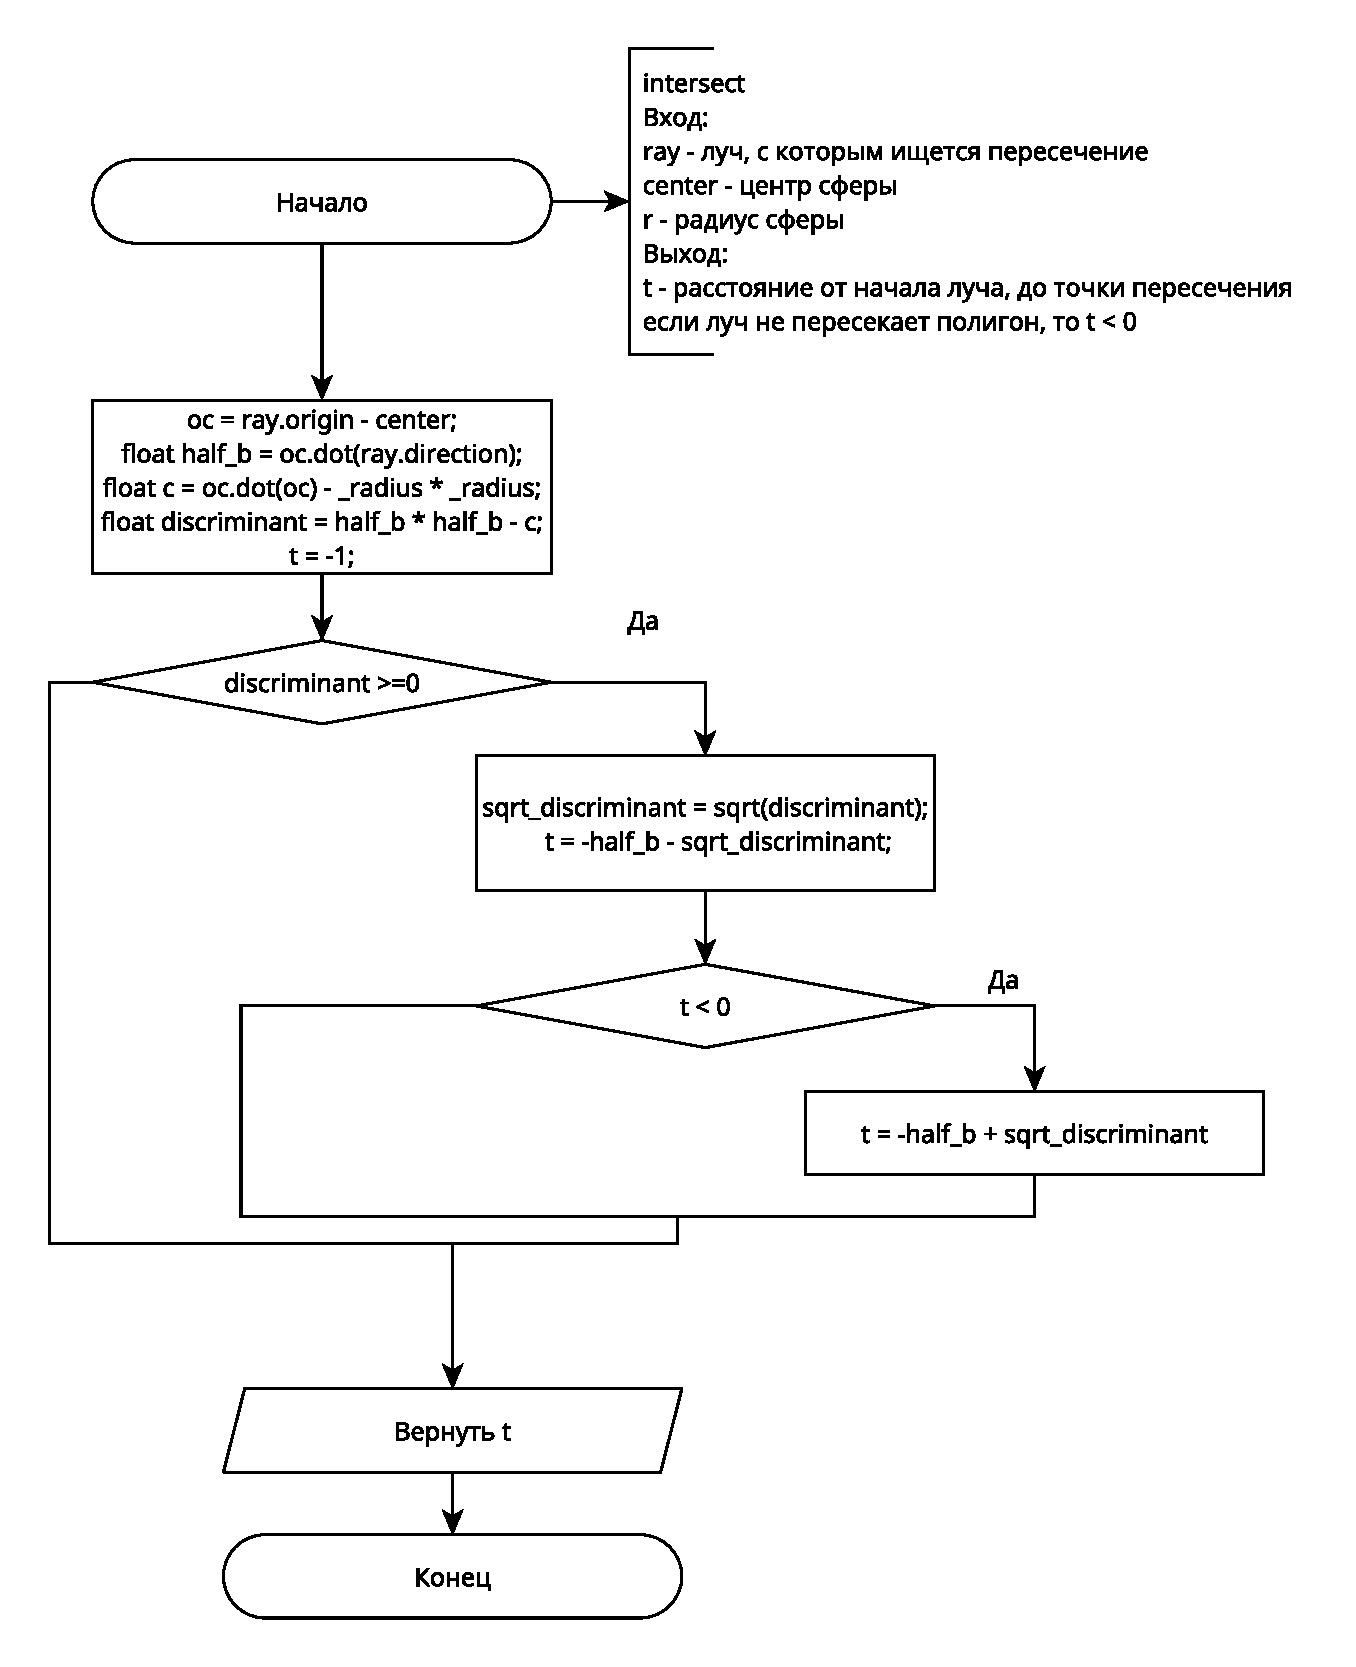
\includegraphics[width=\textwidth, height=210mm, width=170mm, keepaspectratio]{img/sphere_intersect.eps}}
		\caption{Схема алгоритма поиска пересечения с сферой}
		\label{img/sphere_intersect}
	\end{figure}
\subsection{Поиск пересечения луча и полигона}
	Для поиска пересечения луча с треугольным полигоном сначала необходимо проверить, пересекает ли луч плоскость, в которой расположен треугольник. Это можно сделать, проверив, не является ли луч параллельным плоскости, что происходит, если скалярное произведение направления луча и нормали плоскости равно нулю:
\[
(D, n) \neq 0
\]

Если пересечение с плоскостью возможно, вычисляется параметр t, который определяет точку пересечения луча с плоскостью:
\[
t = \frac{(A - V) \cdot n}{(D, n)}
\]
где $A$, $B$ и $C$ — вершины треугольника, $V$ — начальная точка луча, $D$ — направление луча.

Точка пересечения $P$ вычисляется по формуле:
\[
P = V + t \cdot D
\]

После нахождения точки пересечения необходимо проверить, лежит ли она внутри границы треугольника. Для этого задача сводится к двумерному пространству, обнуляя координаты по оси Z у вершин треугольника и точки пересечения.

Затем вычисляются векторные произведения векторов сторон треугольника и векторов, соединяющих первую вершину с точкой пересечения:
\[
v_1 = [AB, AP], \quad v_2 = [BC, BP], \quad v_3 = [CA, CP]
\]

Если все произведения имеют одинаковый знак, то точка пересечения P лежит внутри границы треугольника. Схему алгоритма представлена на рисунке \ref{img/polygon_intersect}
	
	\begin{figure}[H]
		\center{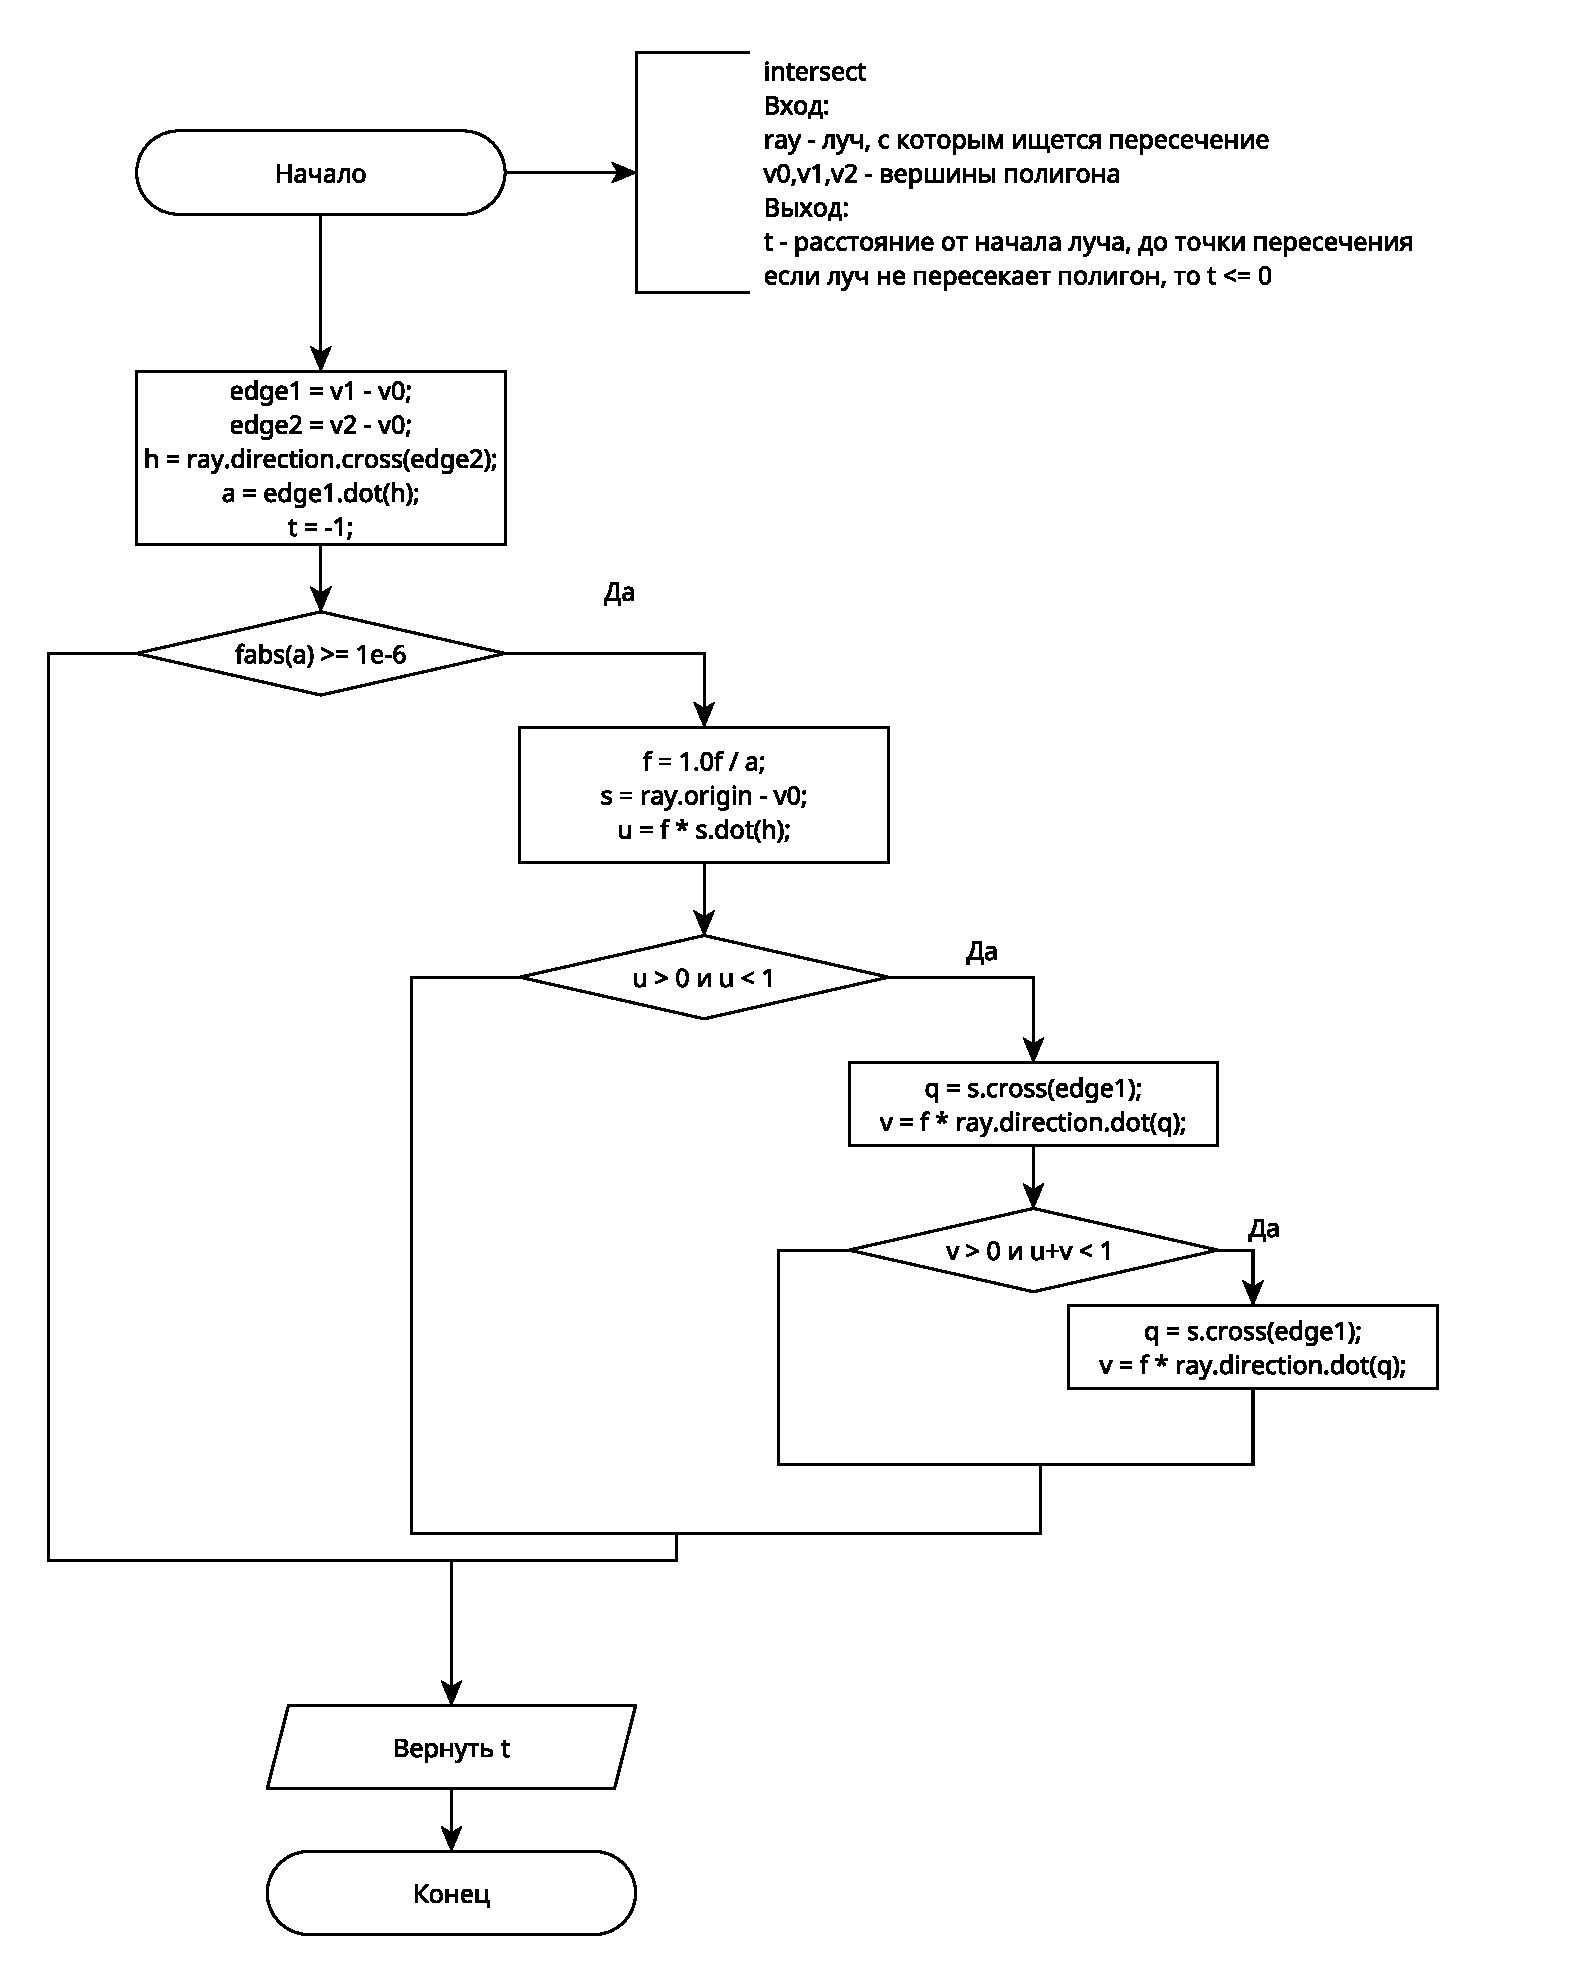
\includegraphics[width=\textwidth, height=210mm, width=170mm, keepaspectratio]{img/polygon_intersect.eps}}
		\caption{Схема алгоритма поиска пересечения с полигоном}
		\label{img/polygon_intersect}
	\end{figure}

\subsection{Персечение с оптической линзой}
Поскольку линза задается пересечением двух сфер, поиск персечения луча с ней сводится к поиск пересечения с этими сферами. Схема алгоритма представлена на рисунке \ref{img/lens_intersect}.
	\begin{figure}[H]
		\center{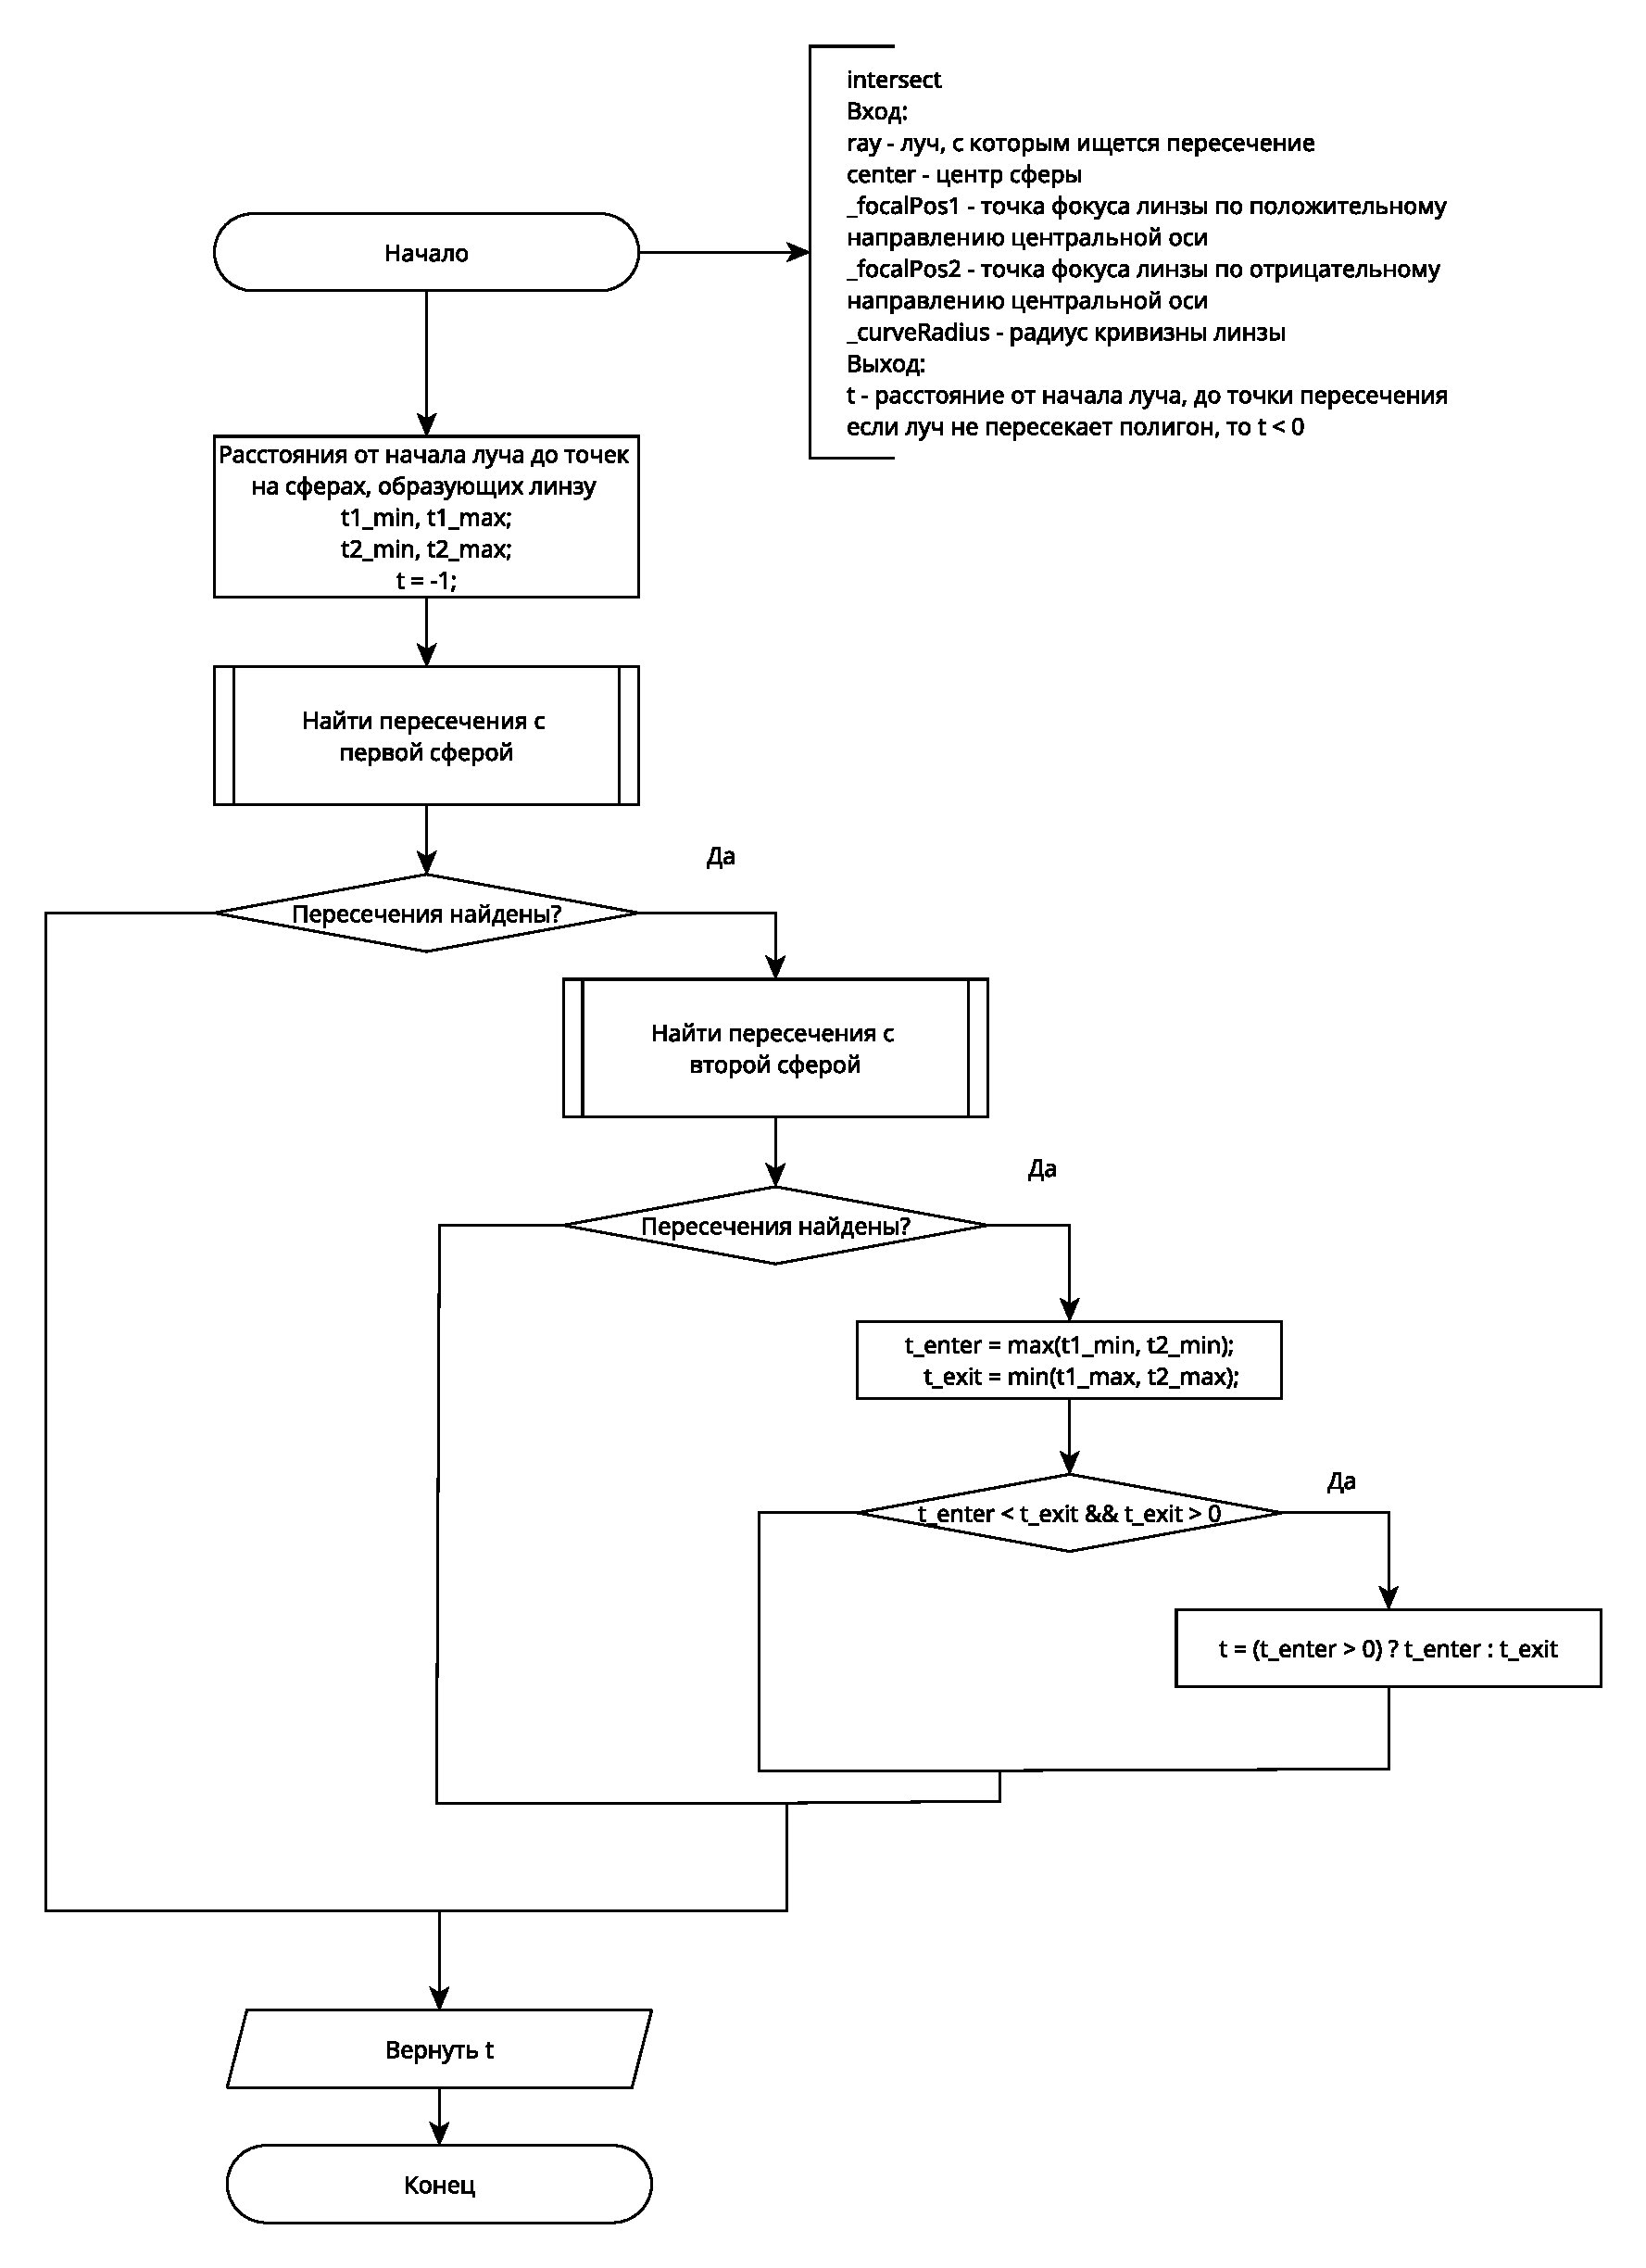
\includegraphics[width=\textwidth, height=210mm, width=170mm, keepaspectratio]{img/lens_intersect.eps}}
		\caption{Схема алгоритма поиска пересечения с линзой}
		\label{img/lens_intersect}
	\end{figure}
	
	\subsection{Обратная трассировка}
	Алгоритм заключается в трассировке лучей от наблюдателя, пока не превысится глубина рекурсивного поиска или луч не будет пересекаться ни с одним объектом сйены. При пересечении с объектом испускается отраженный и преломленный если соответвенно коэффициенты отражения и прозрачности объекта больше 0. Схема алгоритма представлена на рисунках \ref{img/raytracer_1} - \ref{img/raytracer_2}.
	\begin{figure}[H]
		\center{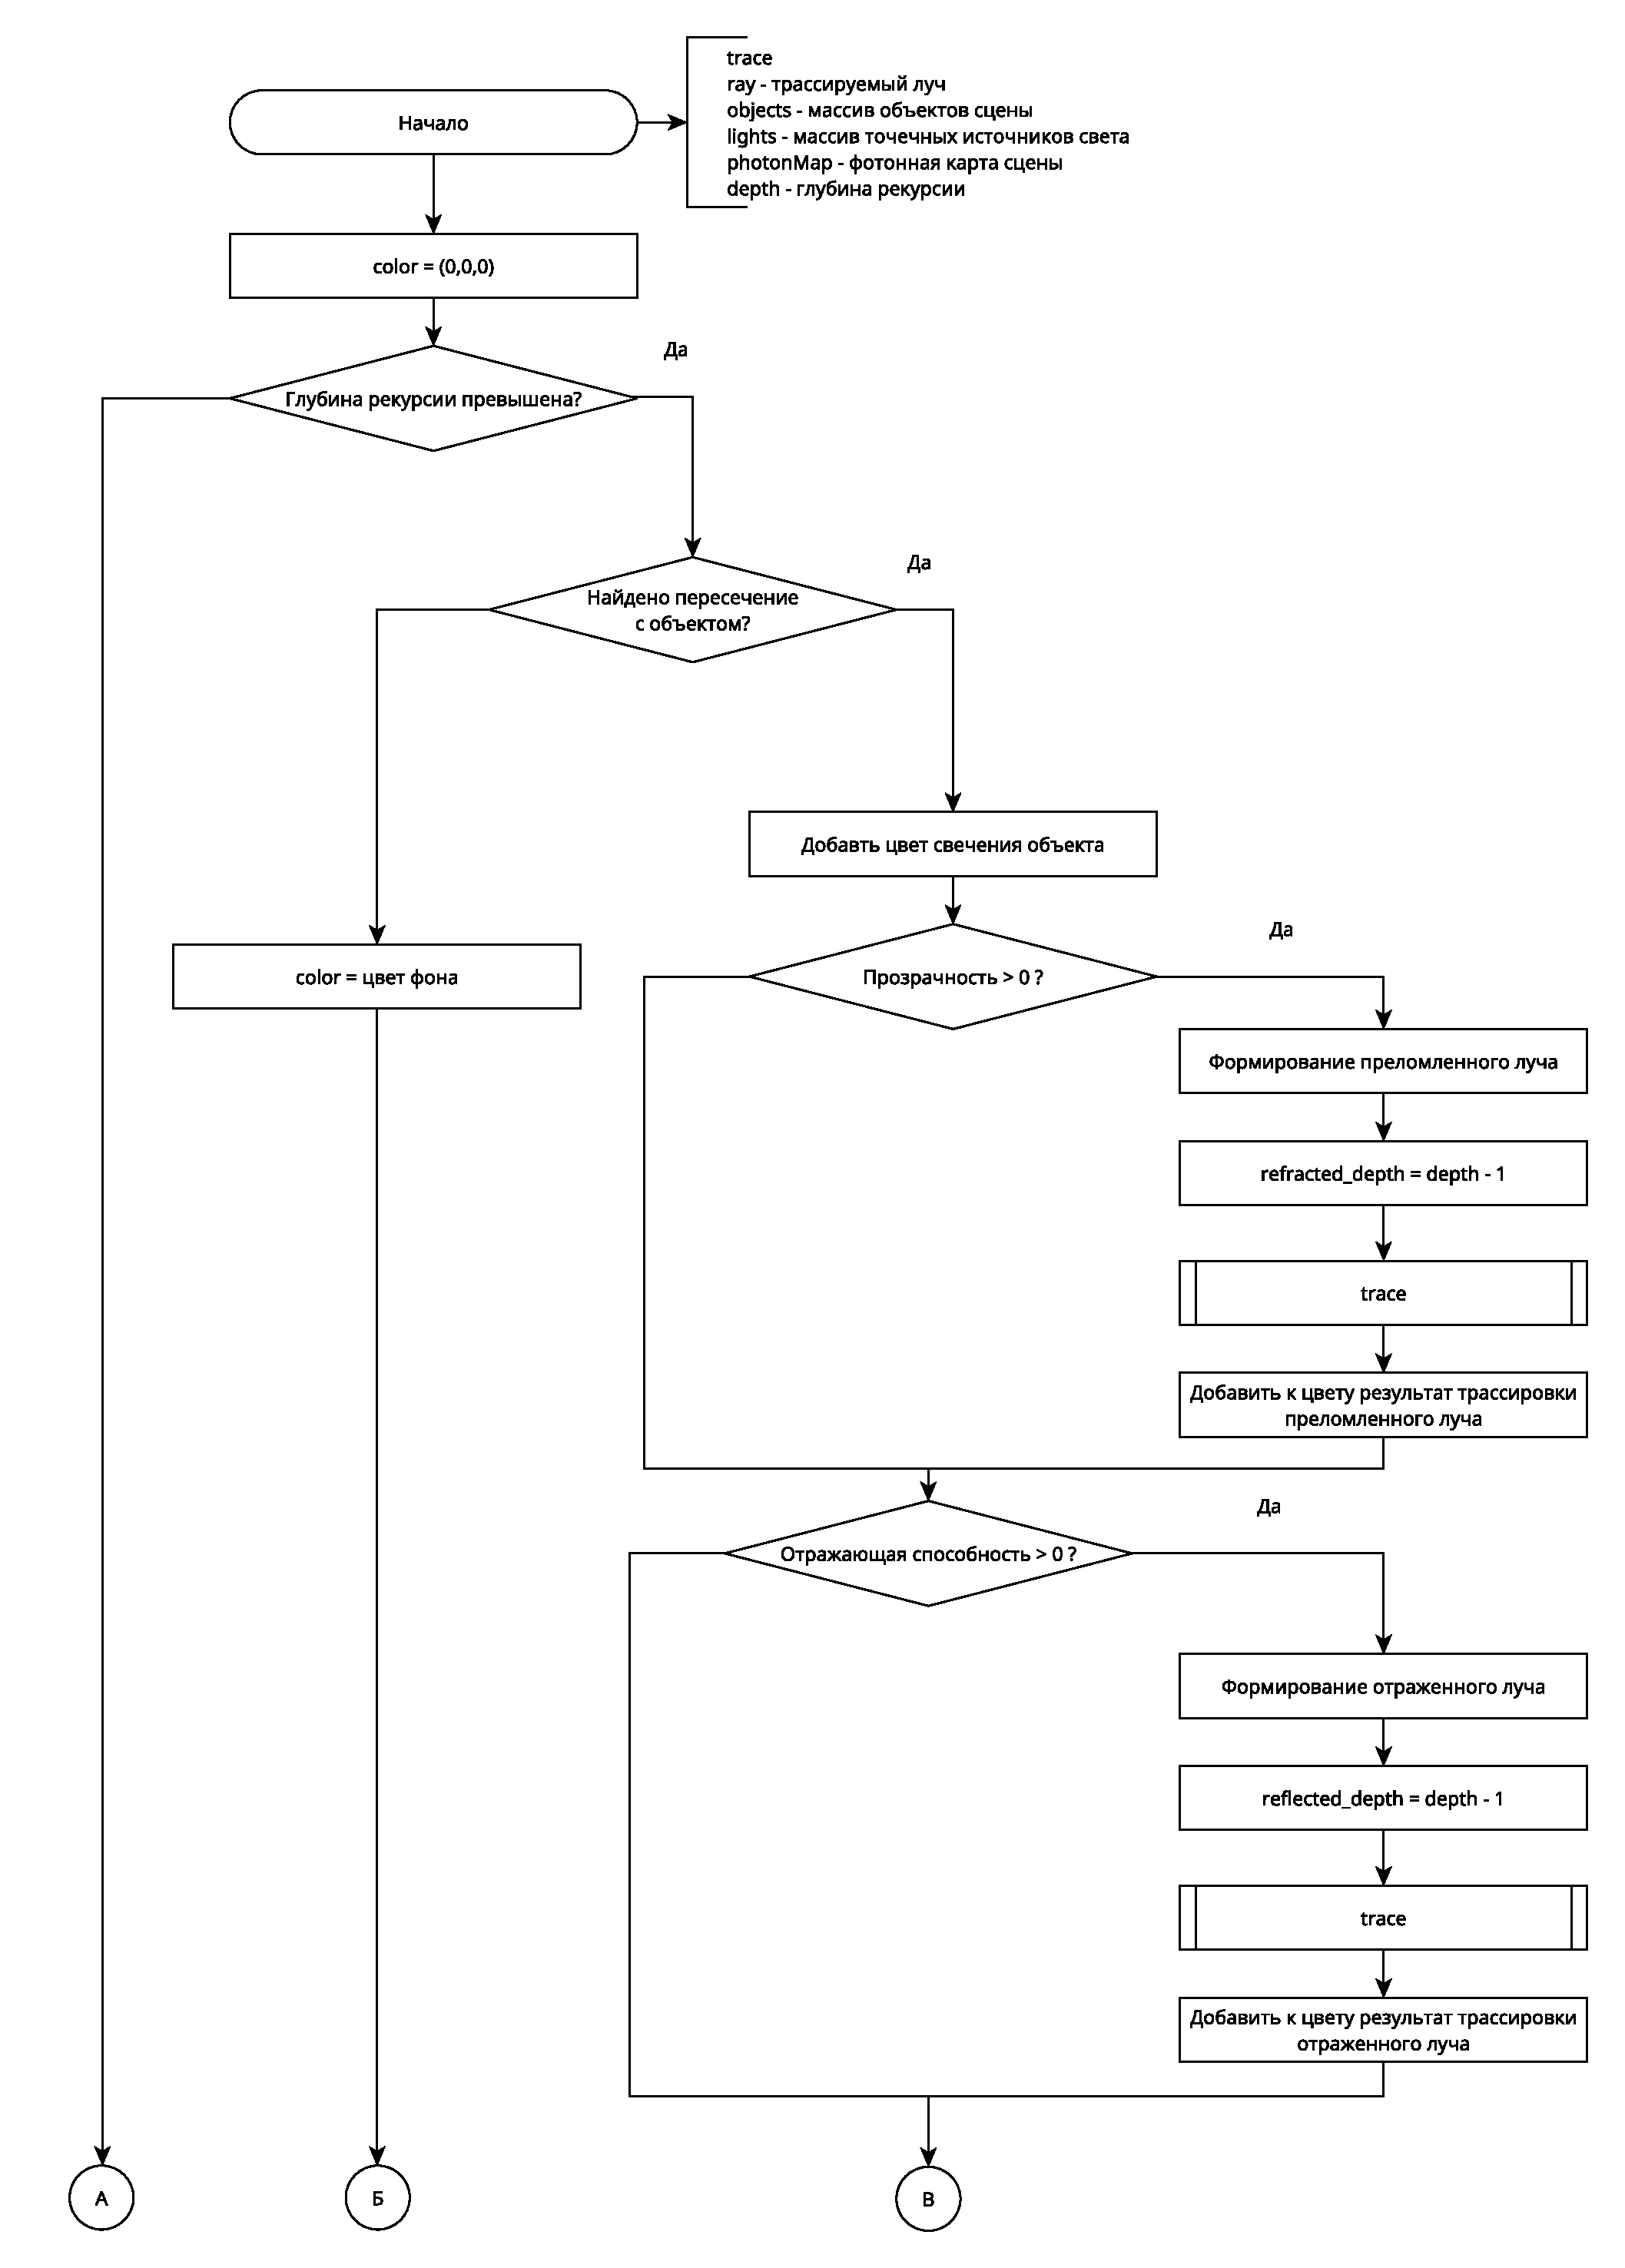
\includegraphics[width=\textwidth, height=210mm, width=170mm, keepaspectratio]{img/raytracer_1.eps}}
		\caption{Схема алгоритма обратной трассировки (часть 1)}
		\label{img/raytracer_1}
	\end{figure}
	
	\begin{figure}[H]
		\center{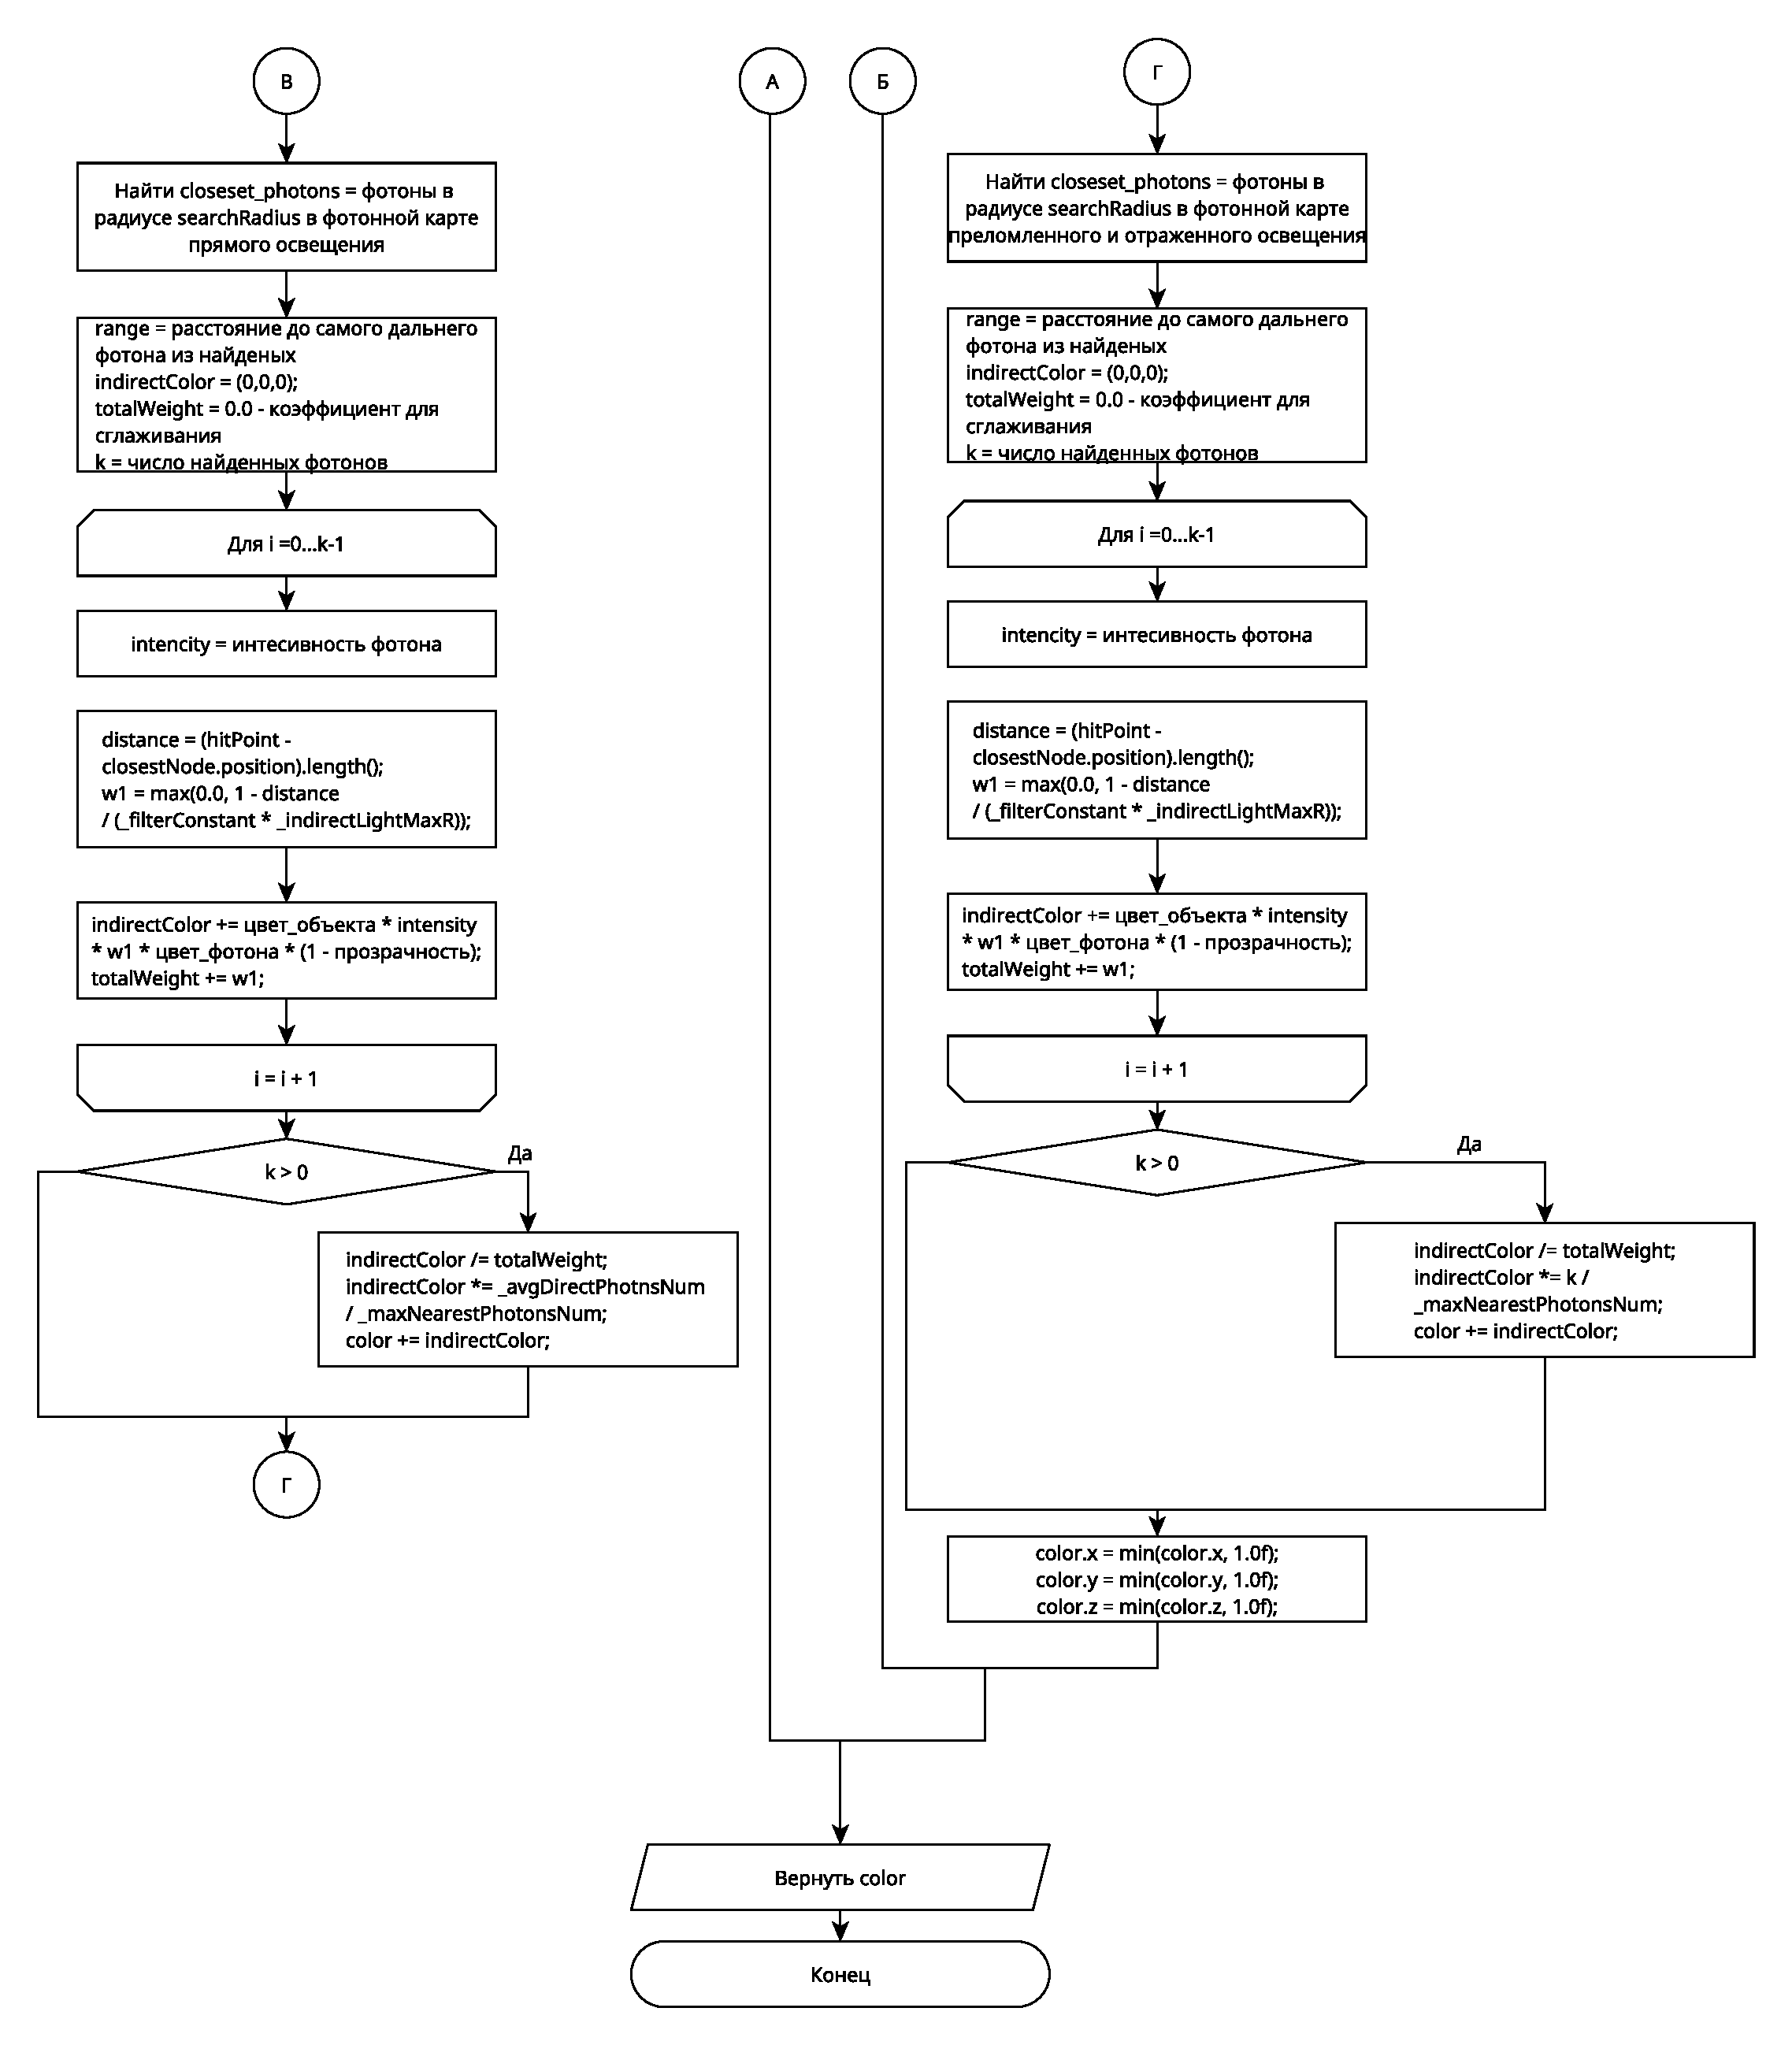
\includegraphics[width=\textwidth, height=210mm, width=170mm, keepaspectratio]{img/raytracer_2.eps}}
		\caption{Схема алгоритма обратной трассировки (часть 2)}
		\label{img/raytracer_2}
	\end{figure}
	
\subsection{Алгоритм построения фотонной карты}

Фотонная карта хранит пересечения фотонов с объектами ввиде K-мерного дерева. При построении карты по списку фотонов список сначала упорядочивается по оси $X$, разбивается пополам, и происходит рекурсивный вызов функции. На следующем шаге рекурсии разбиение происходит по оси $Y$, потом $Z$, посе чего снова по $X$. Схема алгоритма представлена на рисунке \ref{img/photonmap}.
 
	\begin{figure}[H]
		\center{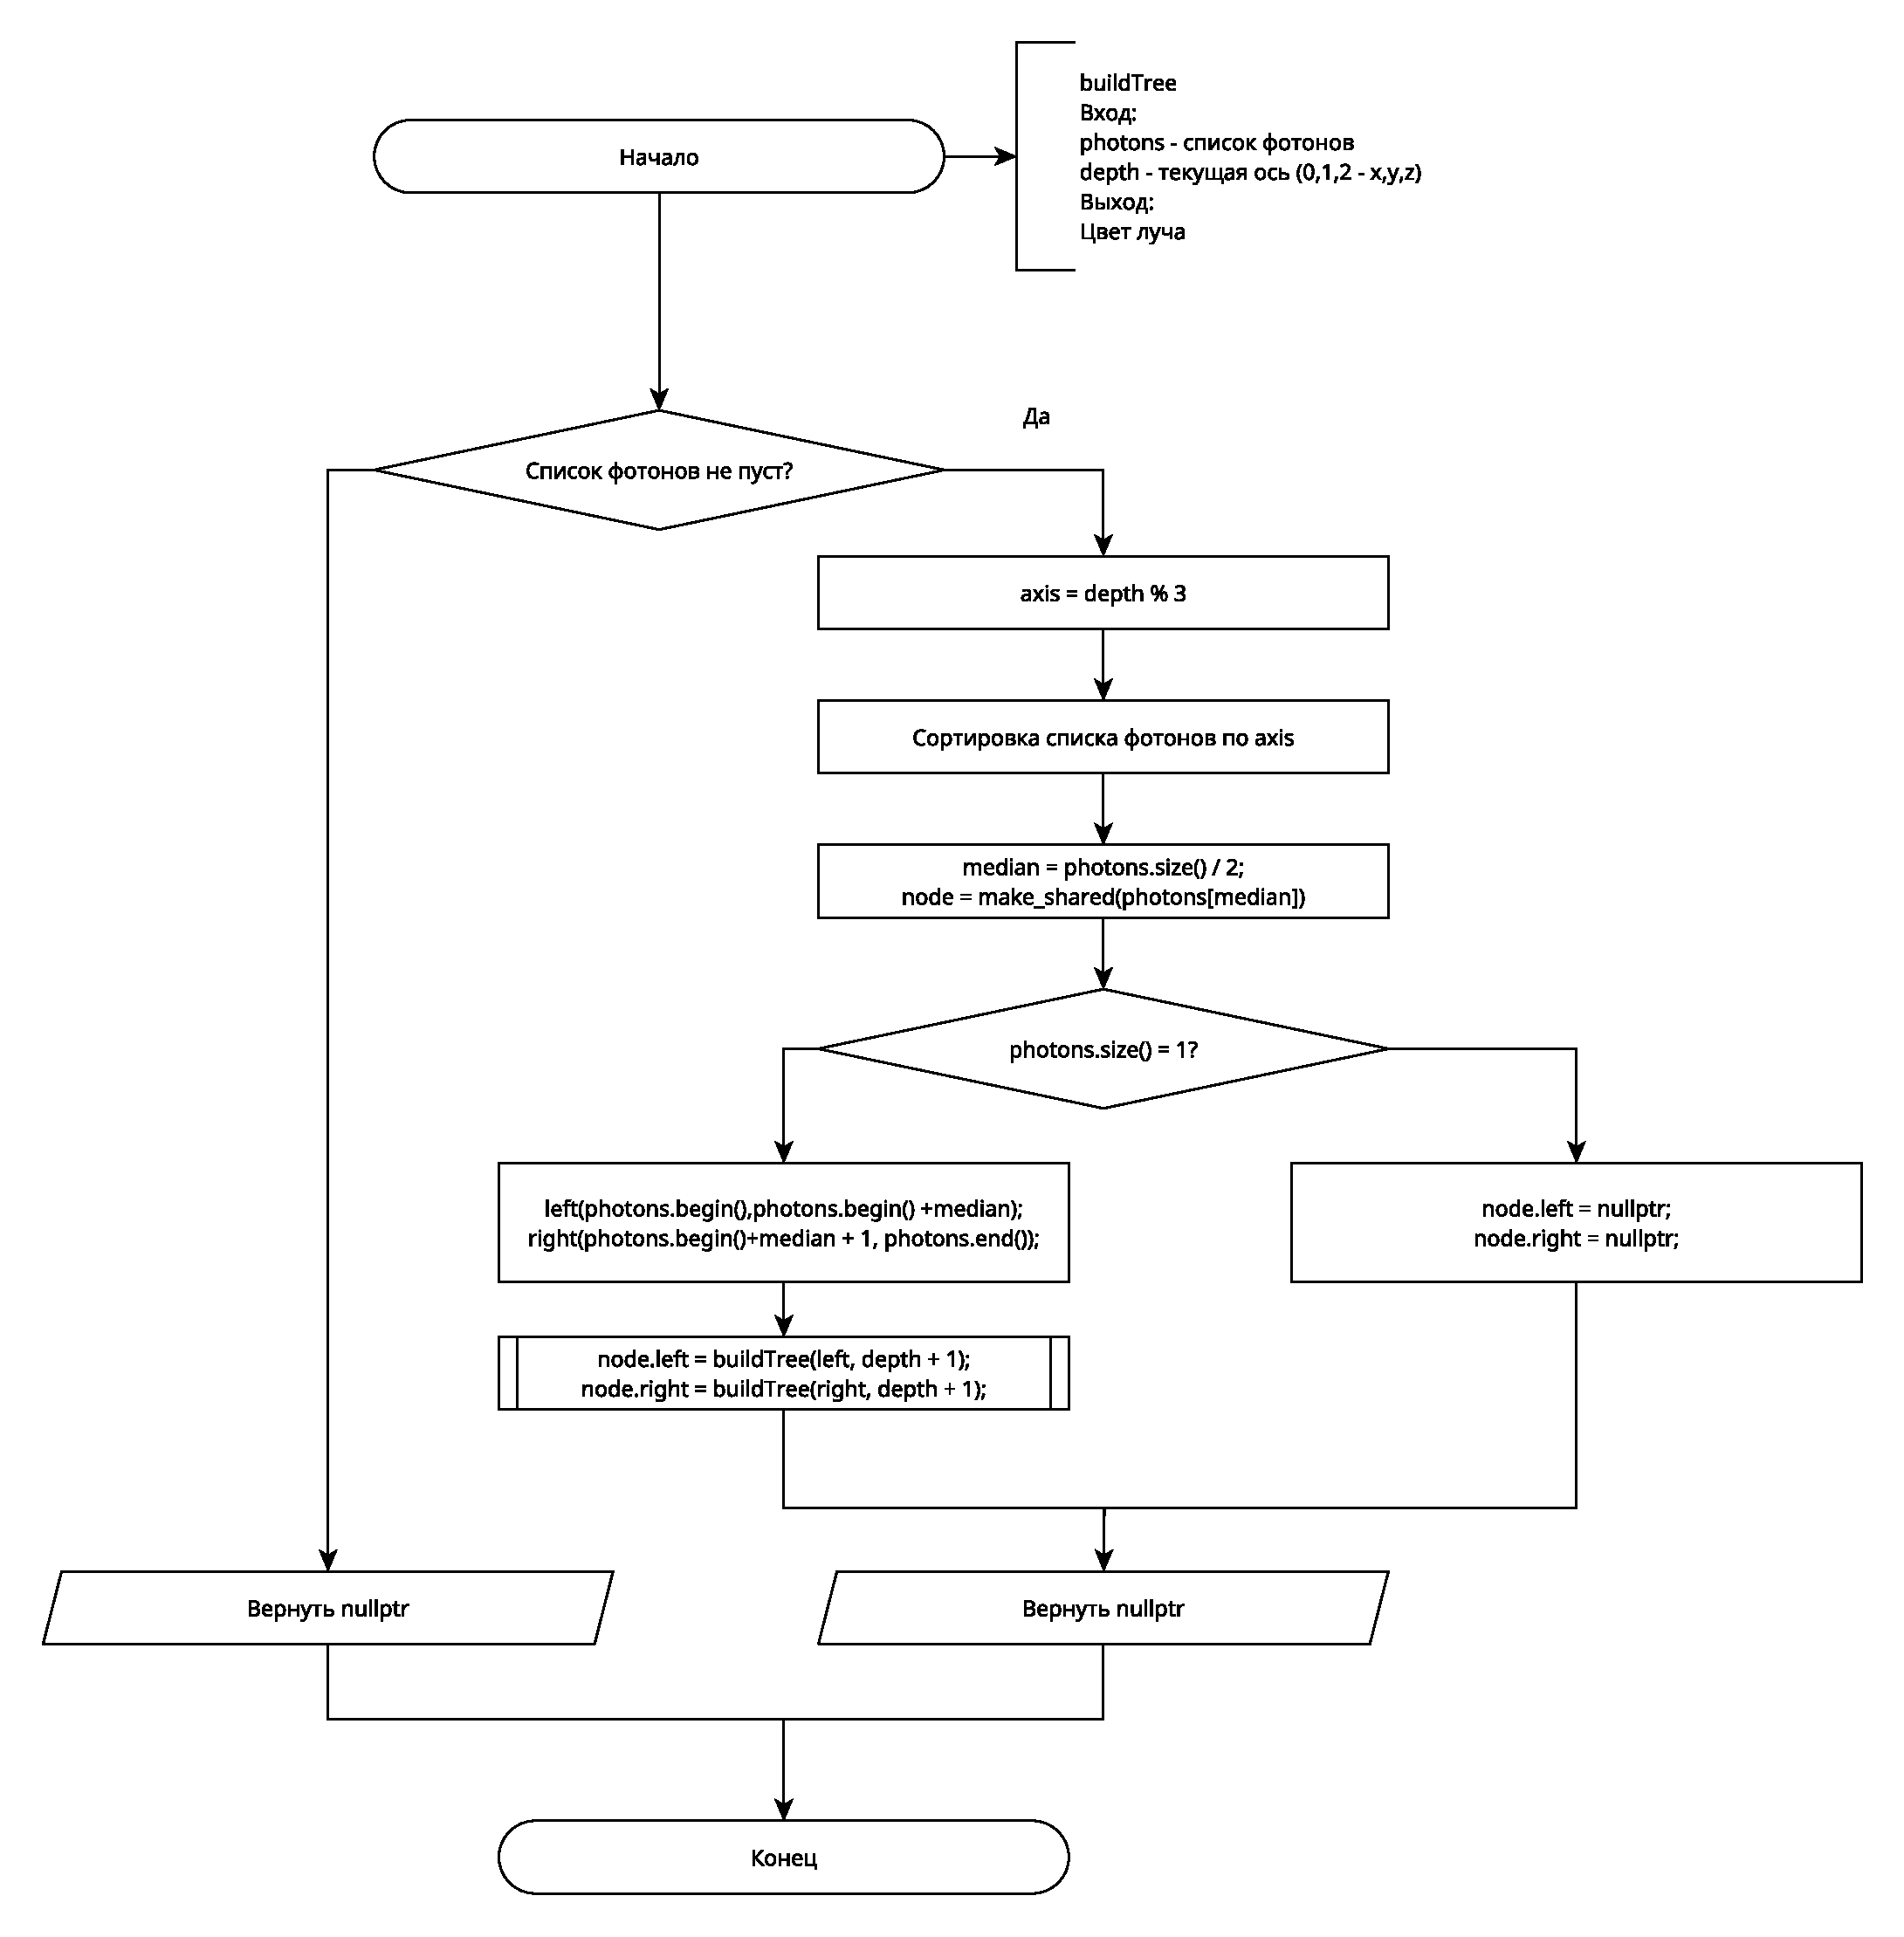
\includegraphics[width=\textwidth, height=210mm, width=170mm, keepaspectratio]{img/photonmap.eps}}
		\caption{Схема алгоритма построения фотонной карты по списку фотонов}
		\label{img/photonmap}
	\end{figure}

	
	